\chapter{Предсказание временного ряда, используя микросервисный подход и потоковую обработку}
\begin{annotation}
  В этой главе будет описана реализация предсказания временного ряда как отдельного сервиса потоковой обработки данных. 
\end{annotation}

\section{Структура}
Прежде всего была определена структура проекта \ref{pic:arch}.

\begin{figure}[!htb]
	\begin{center}
	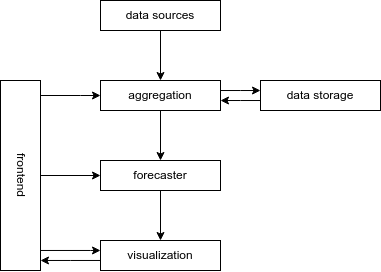
\includegraphics[width=.7\columnwidth]{./img/arch.png}
	\end{center}
	\caption{Схема работы}
	\label{pic:arch}
\end{figure}
\FloatBarrier

Проект состоит из:
\begin{itemize}
  \item data sources - источники данных. В реальности один/несколько распределенных источников данных. В данном примере представлен сервисом, который берет данные из статичного файла.
  \item aggregation - это сервис, собирающий информацию с реальных источников (например точек продаж) в единый агрегированный временной ряд.
  \item forecaster - сервис, получающий части временного ряда и предсказывающий последний, на некоторое время вперед.
  \item visualization - сервис, осуществляющий визуализацию.
  \item frontend - интерфейс для взаимодействия с остальными компонентами.
\end{itemize}


